\documentclass[a4paper,12pt]{article}


\usepackage{graphicx}
\usepackage[ngerman]{babel}

\usepackage{../../exam2e}% lädt unser exam2e.sty
\usepackage{../../mathe2e}% lädt unser math2e.sty


\usepackage{hyperref}

\setlength{\parindent}{1em}
\setlength{\parskip}{0pt}


\begin{document}

\section{Prüfungsaufgaben}


\question%\begin{question}
	Eine Frage mit der Nummer \thequestion
\begin{parts}
	\part Teilaufgabe

	Lorem ipsum\ldots
	\begin{subparts}
		\subpart Unteraufgabe mit Nummer, die so lang ist das ein Zeilenumbruch notwendig wird.

		Außerdem
	\end{subparts}
	\part Nächste Teilaufgabe lautet berechne:%
	\label{part:dieseeineteilaufgabe}
\begin{equation}
	\aaa\quad \frac{1}{2} \qquad\qquad
	\aaa\quad \frac{1}{2} 
\end{equation}
\end{parts}
%\end{question}% Ende von Aufgabe 1
%
\begin{solution}
	Antwort ...
\end{solution}


Text zwischen den Fragen\ldots Eine zweite Frage. Hier folgt als nächste Struktur nicht die Teilaufgabe, sondern gleich die Unteraufgabe. Die Abstände werden automatisch angepasst, die Einstellung des \texttt{parindent} gilt auch für Absätze innerhalb von Fragen.

Ref: wie man in \ref{part:dieseeineteilaufgabe} sehen kann.


\question%\begin{question}
Eine zweite Frage. Hier folgt als nächste Struktur nicht die Teilaufgabe, sondern gleich die Unteraufgabe. Dieses Vorgehen ist in der Unter- und Mittelstufe üblich.

Die Abstände werden automatisch angepasst.
\begin{subparts}
		\subpart Unteraufgabe. Untersuchen Sie  dazu:
	\begin{subsubparts}
		\subsubpart lorem ipsum
		\subsubpart lorem ipsum
	\end{subsubparts}
		\subpart Neue Unteraufgabe. Untersuchen Sie dazu nun:
	\begin{subsubparts}
		\subsubpart lorem ipsum
		\subsubpart lorem ipsum
		\subsubpart lorem ipsum
	\end{subsubparts}
\end{subparts}
%\end{question}
\omitsolution



\question%\begin{question}
	Diese Aufgabe zeigt die ganze Struktur der documentclass \texttt{exam2e}, also question, part, subpart, subsubpart und choice:
\begin{parts}
	\part Teilaufgabe
\begin{subparts}
	\subpart Unteraufgabe
\uplevel{Test von \textbackslash{}uplevel \ldots}
	\subpart Unteraufgabe
	\begin{subsubparts}
		\subsubpart Unterunteraufgabe
	\begin{checkboxes}
		\choice Ankreuzmöglichkeit (alias choice)
	\end{checkboxes}
	\end{subsubparts}
\end{subparts}
\uplevel{Test von \textbackslash{}uplevel \ldots}
	\part Und dann wählen Sie noch hier:
	\begin{checkboxes}
		\choice Ankreuzmöglichkeit 1 \\ mit einem Zeilenumbruch.
		\choice Ankreuzmöglichkeit 2
	\end{checkboxes}
\end{parts}
%\end{question}
\omitsolution




\question[5]%\begin{question}[5]
	Aus einer Tüte mit 
	3 orangenen und 2 gelben Bonbons
%	2 orangenen und 3 gelben Bonbons
	wird zweimal je ein Bonbon gezogen und nicht zurückgelegt.
\begin{subparts}
	\subpart Zeichne ein vollständiges Baumdiagramm.
\uplevel{Nutze das Baumdiagramm zur Beantwortung der folgenden Frage:}%
	\subpart Berechne die Wahrscheinlichkeit zwei verschiedenfarbige Bonbons zu ziehen.
\end{subparts}
%\end{question}

% Lösung zur Aufgabe oben:
\begin{solution}
\begin{subparts}
	\subpart Baumdiagramm:

	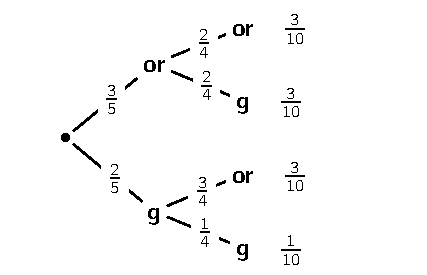
\includegraphics{baumdiagramm}

	\subpart Zu verschiedenfarbig gehören die Fälle von orange-gelb und gelb-orange. In beiden Fällen ist die Wahrscheinlichkeit gleich $\frac{3}{10}$, insgesamt also $\frac{6}{10}$.
\end{subparts}
\end{solution}





   %%%    %%%%%%%%  %%%% 
  %% %%   %%     %%  %%  
 %%   %%  %%     %%  %%  
%%     %% %%%%%%%%   %%  
%%%%%%%%% %%     %%  %%  
%%     %% %%     %%  %%  
%%     %% %%%%%%%%  %%%% 

\section{Abituraufgaben}

Hier ist noch die Neudefinition von \texttt{subpart} einzufügen, damit die Unteraufgaben fortlaufend mit 1.1.1 usw. durchnummeriert werden.

Durch den neuen Abschnitt werden die Aufgabenzähler zurückgesetzt.

\subsubsection*{Eine abiturähnliche Aufgabe}
\titledquestion{Der Titel der Aufgabe:} Dies ist dann der Text der Aufgabe.
\begin{parts}
\part asdf
\begin{subparts}
	\subpart asdf
	\subpart asdf
\end{subparts}
\part
\begin{subparts}
	\subpart Nummerierung ohne einleitenden Text
	\subpart asdf
\end{subparts}
\end{parts}



\subsubsection*{Eine zweite abiturähnliche Aufgabe}

\question asdf
\begin{parts}
	\part asdf
	\part asdf
	\part asdf
	\part asdf
\end{parts}


\end{document}




